\documentclass{article}
\usepackage[utf8x]{inputenc}
\usepackage{tikz}

\begin{document}

\section{Trasee formate din linii drepte}

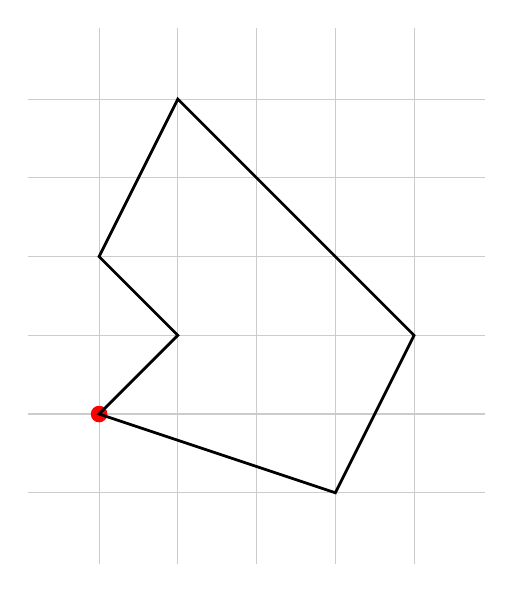
\begin{tikzpicture}[x=1cm,y=1cm]
  % grilă cu pasul de discretizare 1x1
  \draw[help lines,thin,gray!40] (-0.9,-1.9) grid (4.9,4.9);
  % punctul (0,0) 
  \fill[red] (0,0) circle (3pt);
  
  % poligon
  \draw[line width=1pt] (0,0) -- (3,-1) -- (4,1) -- (1,4) -- (0,2) -- (1,1) -- cycle;
\end{tikzpicture}
%
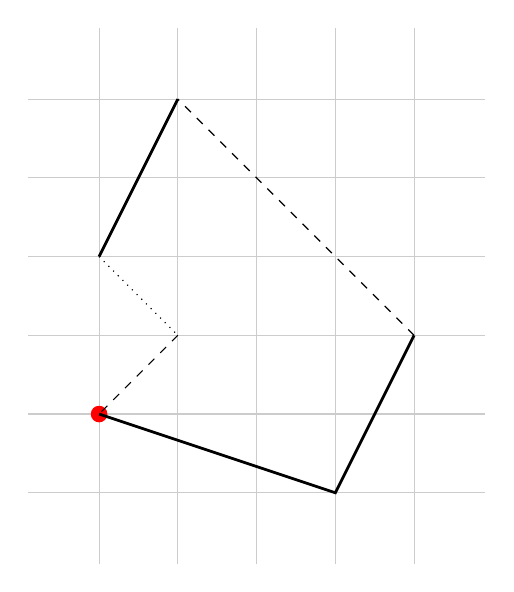
\begin{tikzpicture}[x=1cm,y=1cm]
  % grilă
  \draw[help lines,thin,gray!40] (-0.9,-1.9) grid (4.9,4.9);
  % punctul (0,0) 
  \fill[red] (0,0) circle (3pt);
  
  % linii neîntrerupte  
  \draw[line width=1pt] (0,0) -- (3,-1) -- (4,1) (1,4) -- (0,2);
  % linii întrerupte
  \draw[dashed] (4,1) -- (1,4) (1,1) -- (0,0);
  % linie punctată
  \draw[dotted] (0,2) -- (1,1);
\end{tikzpicture}

\newpage

\section{Trasee formate din linii drepte și curbe}

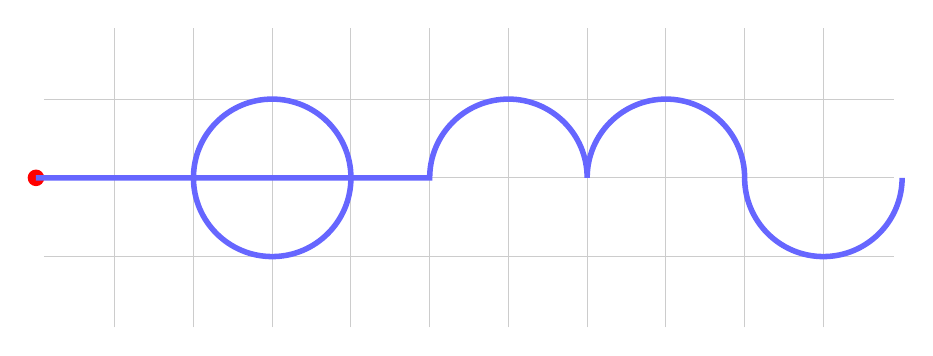
\begin{tikzpicture}[x=1cm,y=1cm]
  % grilă
  \draw[help lines,thin,gray!40] (0.1,-1.9) grid (10.9,1.9);
  % punctul (0,0) 
  \fill[red] (0,0) circle (3pt);
  
  \draw[color=blue!60, line width=2pt] (0,0) -- (3,0) circle (1) -- (5,0) arc (180:0:1) arc (180:0:1) arc (180:360:1);
\end{tikzpicture}

\newpage

\section{Etichetarea punctelor de pe traseu}

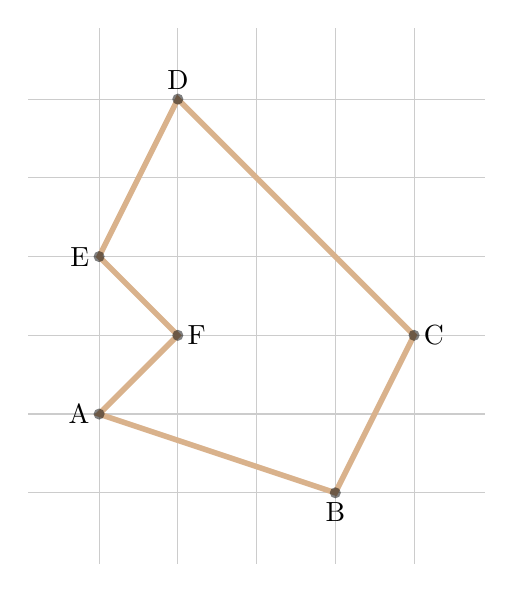
\begin{tikzpicture}
  % grilă
  \draw[help lines,thin,gray!40] (-0.9,-1.9) grid (4.9,4.9);
  
  % specificarea coordonatelor
  \coordinate[label=left:A] (A) at (0,0);
  \coordinate[label=below:B] (B) at (3,-1);
  \coordinate[label=right:C] (C) at (4,1);
  \coordinate[label=D] (D) at (1,4);
  \coordinate[label=left:E] (E) at (0,2);
  \coordinate[label=right:F] (F) at (1,1);
  
  % poligon
  \draw[line width=2pt,color=brown!60] (A) -- (B) -- (C) -- (D) -- (E) -- (F) -- cycle;
  
  % desenarea punctelor
  \foreach \point in {A,B,C,D,E,F}
    \fill [black,opacity=.5] (\point) circle (2pt);
\end{tikzpicture}

\textbf{1 Exercițiu:} Pentru poligonul $ABCDEF$, din figura de mai sus, construiți  diagonalele cu linii întrerupte.

\newpage

\section{Automatizarea construcției desenelor TikZ cu ajutorul ciclurilor (sau Apropo de \emph{foreach}...)}

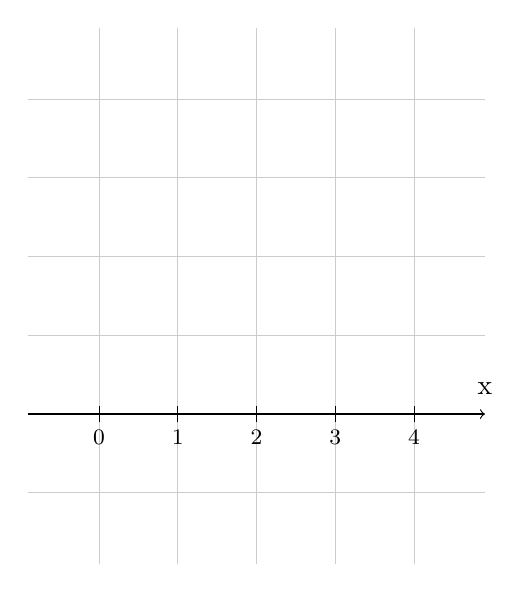
\begin{tikzpicture}
  % grilă
  \draw[help lines,thin,gray!40] (-0.9,-1.9) grid (4.9,4.9);
  % axa 'x'
  \draw[->] (-0.9,0) -- (4.9,0) node[label=above:x] (x) {};

  % diviziunile (de la 0 la 4) ale axei 'x'
  \foreach \x in {0,...,4}
  {
    \draw (\x,0.1) -- (\x,-0.1);
    \node at (\x,-0.3) {\footnotesize{\x}};
  }  
\end{tikzpicture}

\textbf{2 Exeercițiu:} Construiți cealaltă axă.

\newpage

\section{Coordonate polare}

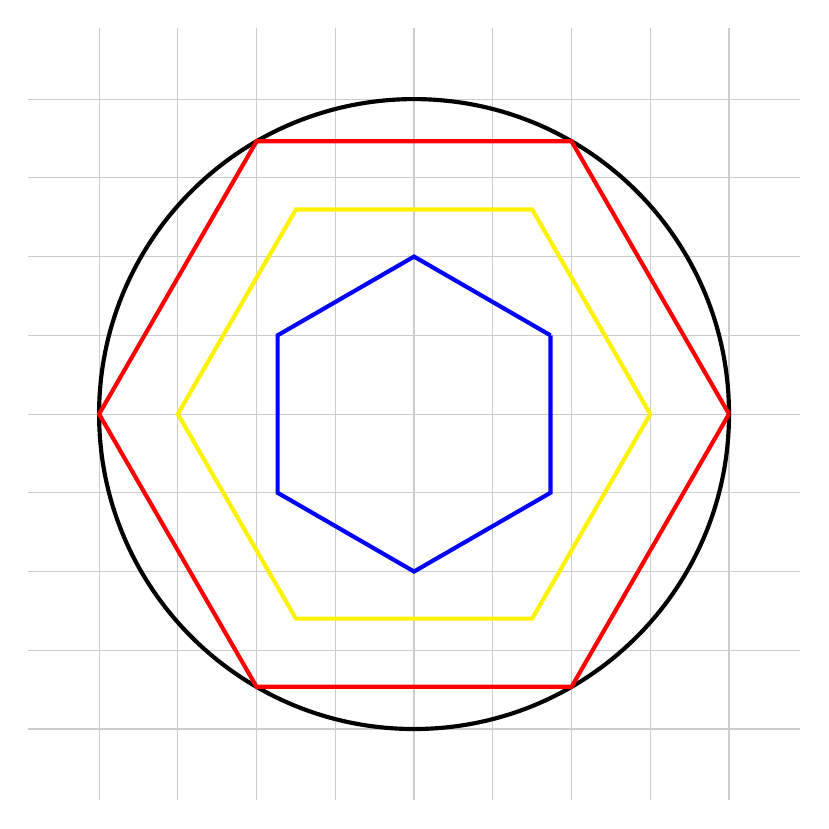
\begin{tikzpicture}
  % grilă
  \draw[help lines,thin,gray!40] (-4.9,-4.9) grid (4.9,4.9);
  
  % cerc de raza 4
  \draw[line width=1.5pt] (0,0) circle (4);
  % hezagon înscris în cerc
  \draw[line width=1.5pt,color=red] (0:4) -- (60:4) -- (120:4) -- (180:4) -- (240:4) -- (300:4) -- (360:4);
  %hexagon înscris în cercul de raza 3
  \draw[line width=1.5pt,color=yellow] (0:3) -- (60:3) -- (120:3) -- (180:3) -- (240:3) -- (300:3) -- (360:3);  
  % hexagon înscris în cercul de raza 2, rotit cu 30 grade 
  \draw[rotate=30,line width=1.5pt,color=blue] (0:2) -- (60:2) -- (120:2) -- (180:2) -- (240:2) -- (300:2) -- (360:2);
\end{tikzpicture}

\textbf{3 Exercițiu:} Construți un triunghi echilateral inscris în acest cerc.

\section{Coordonate relative}

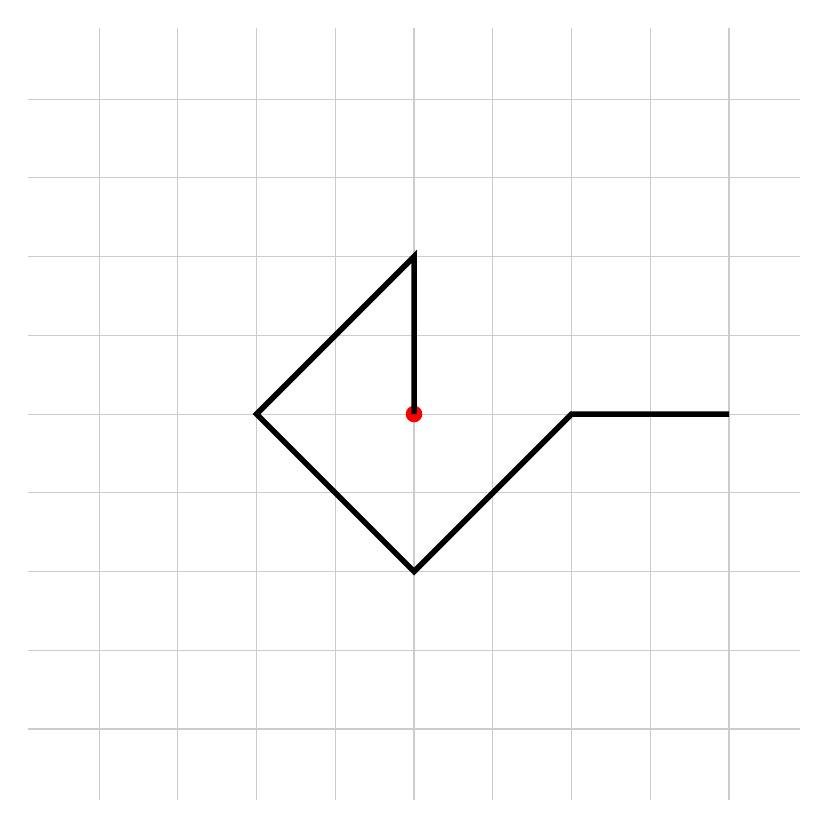
\begin{tikzpicture}
  % grilă
  \draw[help lines,thin,gray!40] (-4.9,-4.9) grid (4.9,4.9);
  % punctul (0,0) 
  \fill[red] (0,0) circle (3pt);
  
  \draw[line width=2pt] (0,0) -- +(0,2) -- +(-2,0) -- +(0,-2) -- ++(2,0) -- +(2,0);
\end{tikzpicture}

\end{document}